\newpage
\section{Methodology}

\subsection{Design Methods and Development Strategy}

\subsubsection{Design-Based Research}

Design-based research (DBR) is a research methodology aimed at improving educational practices through systematic, flexible, and iterative processes of analysis, design, development, implementation, and evaluation. It is grounded in collaboration between researchers and practitioners in real-world settings, ultimately producing design principles or theoretical contributions \parencite{wang_influence_2026}.

DBR is primarily conducted in authentic educational environments to bridge the gap between theoretical research and practical application \parencite{jong_design-based_2017}. Unlike traditional laboratory-based approaches, DBR is situated in naturalistic contexts where social interactions and environmental complexity are preserved and considered as integral parts of the research process \parencite{wang_influence_2026}.

A central feature of DBR is its iterative cycle, which consists of design, enactment, analysis, and redesign illustrated in \cref{fig:dbr_cycle}. The outputs of each cycle inform and guide subsequent cycles, enabling continuous refinement of both the intervention and the underlying theory \parencite{jong_design-based_2017}.


\begin{figure}[H]
\caption{Iterative cycle of Design-Based Research}\label{fig:dbr_cycle}
\centering
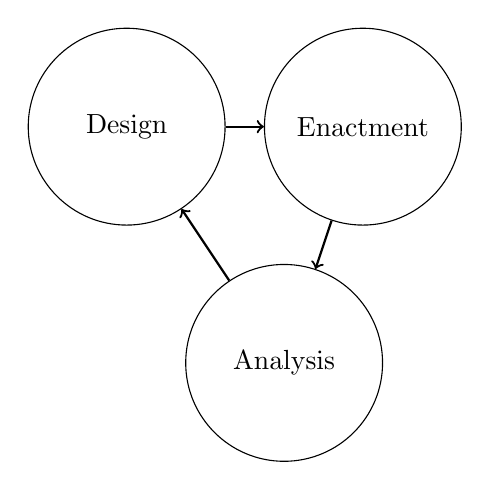
\begin{tikzpicture}[
    every node/.style={draw, circle, minimum size=2.5cm, align=center},
    arrow/.style={->, thick}
]

\node (design) at (0,0) {Design};
\node (enact) at (3,0) {Enactment};
\node (analysis) at (2,-3) {Analysis};

\draw[arrow] (design) -- (enact);
\draw[arrow] (enact) -- (analysis);
\draw[arrow] (analysis) -- (design);

\end{tikzpicture}
\end{figure}
\textcite{Beck2004XP} define Agile as a set of values and principles that emphasize iterative development, customer collaboration, and responsiveness to change. Agile development approaches typically include iterative and incremental development, self-organizing teams, and continuous feedback and adaptation.

Agile processes focus on the rapid and early delivery of working software and are based on development models that support incremental and iterative progress \parencite{keith2010agile}.

A user story is a description of a feature expressed from the perspective of the user and its intended value. User stories serve as the core unit of work in Agile development. Multiple user stories are maintained in a backlog, from which a subset is selected for implementation during a time-boxed iteration, typically lasting two to four weeks, known as a sprint. A collection of related user stories that collectively deliver a larger functional capability is referred to as an epic. Completed sets of functionality, such as alpha or beta versions, are commonly referred to as milestones.

User stories must be estimated, which requires sufficient understanding of both the system being built and the implementation approach. If the scope of a story is too large or insufficiently understood, accurate estimation becomes difficult. Such cases are often addressed through spikes, which are time-boxed research tasks used to reduce uncertainty \parencite{keith2010agile}.

Both DBR and Agile share a common iterative philosophy, in which development proceeds through cycles of analysis, implementation, evaluation, and refinement, enabling continuous learning and adaptation throughout the process.

\subsubsection{Development Strategy}

This study includes three objectives in development, (1) Choosing or implement an FPV quadcopter physics; (2) Implement and testing a human-AI collaboration agent; (3) Choosing a set of interaction UI components and implement the XR environment.

% TODO: undone

\subsection{Development Environment and Materials}

\subsubsection{Comparison of Development Platforms}

Game development is strongly influenced by the choice of game engine. Before initiating a project, it is critical to determine the target hardware and environmental requirements, as these factors define the development constraints.

This section presents a comparison of current game engines supporting extended reality, based on programming language, physics engine, rendering methods, Meta platform support, machine learning support, and editor size (see Table~\ref{table:xr_engine}). This comparison is based on official documentation and prior research from \parencite{ezhil_comparative_nodate}.

\begin{table}[h]
\centering
\caption{Software Engine Comparison}\label{table:xr_engine}
\setlength{\tabcolsep}{6pt} 
\begin{tabularx}{1\textwidth}{l|X|X|X|X}
\hline
Feature & Unreal Engine (5.7) & Unity (6.0) & Godot (4.6) & Wonderland Engine \\
\hline
Language & C++, Blueprints    & C\#        & GDScript, C\# & JavaScript, TypeScript \\
Physics & Chaos Physics      & NVIDIA PhysX, DOTS & Jolt Physics   & NVIDIA PhysX \\
Rendering  & Lumen, Nanite & URP, HDRP    & Forward+, Mobile & WebGL2 \\
Meta Support & Fork build  & First-class & Community-driven & No support \\
ML Support & Learning Agent & ML Agents & Godot RL Agents & No support \\
Editor Size & $\sim$50GB+ & $\sim$20GB & $<1$GB & 200MB \\
\hline
\end{tabularx}

\end{table}

Unreal Engine: Unreal Engine is widely recognized for its photorealistic rendering capabilities and high visual fidelity. Its Chaos Physics engine is highly regarded for complex simulations, making it the foundation for projects like Microsoft's AirSim. However, UE has a high barrier to entry: the editor is massive, and utilizing Meta's private APIs often requires compiling a custom engine branch from source.

Unity: Unity remains the most popular choice for Meta Quest development due to its mature SDK support and C\# scripting. While it uses PhysX by default, its DOTS (Data-Oriented Technology Stack) provides high-performance physics for complex drone swarms. It offers the most streamlined out-of-the-box experience for Standalone VR.

Godot: Godot has emerged as a powerful, lightweight alternative. It is highly compatible with modern AI coding assistants due to its Python-like GDScript. The integration of Jolt Physics as the default 3D engine has resolved previous performance hurdles for VR. However, its XR ecosystem is largely community-maintained. While excellent for prototyping, the lack of official Meta API support and the potential instability of third-party GDExtensions require careful dependency management for production-grade projects.

Wonderland Engine: Wonderland Engine is a specialized WebXR engine built in C++ and compiled to WebAssembly.  By leveraging WebGL2, it achieves the performance necessary to render thousands of objects at native frame rates directly within a browser. The development workflow relies on JavaScript and TypeScript, providing a highly familiar and accessible environment for traditional web developers. A unique advantage is the ability to edit scenes directly on the headset, enabling instant feedback without removing the device.

Unity 3D is frequently used in research due to its flexible configuration, extensive plugin ecosystem, and ease of rapid prototyping. Thus, it is often used in various experiments \parencite{shatokhin_extended_2025}.



\subsubsection{Materials and Equipment: Game Assets, AI, Development Tools}

%TODO!



% Object: Drone Physics

\subsection{Simulate the Quadcopter}

This section examines the flight dynamics and control implementation
found in the Yue's Ultimate Drone physics model \parencite{yuetility2022fpvphysics}. 

\subsubsection{Controller Mapping}

The flight controller distinguishes between unipolar throttle inputs and bipolar command sticks (Roll, Pitch, and Yaw): Throttle ($T$): Mapped to a normalized range of $[0, 1]$. Attitude Commands ($\theta, \phi, \psi$): Mapped to a range of $[-1, 1]$.

To refine the pilot's control over the aircraft, the system utilizes a non-linear control curve for joystick calculation. As \parencite{lovesay2003ergonomics} observes, a good quality force tracking controller has a linear output, with joystick force directly proportional to sight velocity, but many systems shape the joystick voltage output, to achieve fine control and greater tracking accuracy as the joystick output approaches zero, whilst retaining the same maximum output capability.

In this implementation, shaping is achieved by combining proportional ($p$) and exponential ($e$) components to calculate the target angular rate ($\tau$) from the raw angular rate ($u$) as shown in \cref{eq:mapping}.

\begin{equation}\label{eq:mapping}
    \tau = p \cdot u + e \cdot \text{sgn}(u) \cdot u^{2}
\end{equation}

The raw gamepad throttle $u_T \in [-1, 1]$ is normalized to a linear thrust scalar as shown in \cref{eq:mappingt}

\begin{equation}\label{eq:mappingt}
    T = \frac{u_T + 1}{2}
\end{equation}

\subsubsection{Flight Modes and Orientation Logic}

Since the Unity engine utilizes the FixedUpdate method for physics calculations, the drone's target orientation is updated discretely at every physics timestep ($\Delta t$).

In Acro mode, the joystick inputs command the angular rate of change. The drone's target orientation $q_{\text{target}}$ is an accumulation of these rates over time. The orientation is updated by integrating the processed angular rates ($\tau_\phi, \tau_\theta, \tau_\psi$) as shown in \cref{target_angular}, the Quaternion.Euler equation is \cref{eq:torque}.

\begin{equation}\label{target_angular}
\begin{gathered}
    q_{\Delta} = \text{Quaternion.Euler}(\tau_\theta \Delta t, \tau_\phi \Delta t, \tau_\psi \Delta t) \\
    q_{\text{target}, k} = q_{\text{target}, k-1} \cdot q_{\Delta}
\end{gathered}
\end{equation}

In Self-Leveling mode, intended to prevent crashing and ease navigation, the pitch and roll sticks command a specific angle rather than a rate. Given a predefined maximum bank angle for pitch ($\theta_{\max}$) and roll ($\phi_{\max}$), the target values are calculated as \cref{eq:leveling}.

\begin{equation}\label{eq:leveling}
  \theta_{\text{target}} = u_\theta \cdot \theta_{\max}, \quad \phi_{\text{target}} = u_\phi \cdot \phi_{\max}  
\end{equation}

The simulation applies two primary vectors to the drone's Rigidbody: appliedForce (Thrust) and appliedTorque (Attitude Control).

The total thrust force $\mathbf{F}_{\text{thrust}}$ is applied along the vehicle's local up vector ($\hat{\mathbf{u}}_{\text{up}}$). The magnitude is governed by the throttle $T$ and the maximum thrust constant $F_{\max}$, the thrust force is calculated as shown in \cref{eq:force}.

\begin{equation}\label{eq:force}
    \mathbf{F}_{\text{thrust}} = (T \cdot F_{\max}) \cdot \hat{\mathbf{u}}_{\text{up}}
\end{equation}


% Object: AI for learning
\subsection{Design of the Human-AI Collaboration}

\subsubsection{Design of a PD based CO-Trainer}

Proportional integral derivative (PID) shown in \cref{eq:pid} can be applied for making a simple aviation helper in piloting the quadcopter. For basic flight stabilization, a simple PD action can provide satisfactory performance shown in \cref{fig:pd}.

\begin{figure}
    \caption{Comparison of PID and PD}\label{fig:pd}
    \centering
    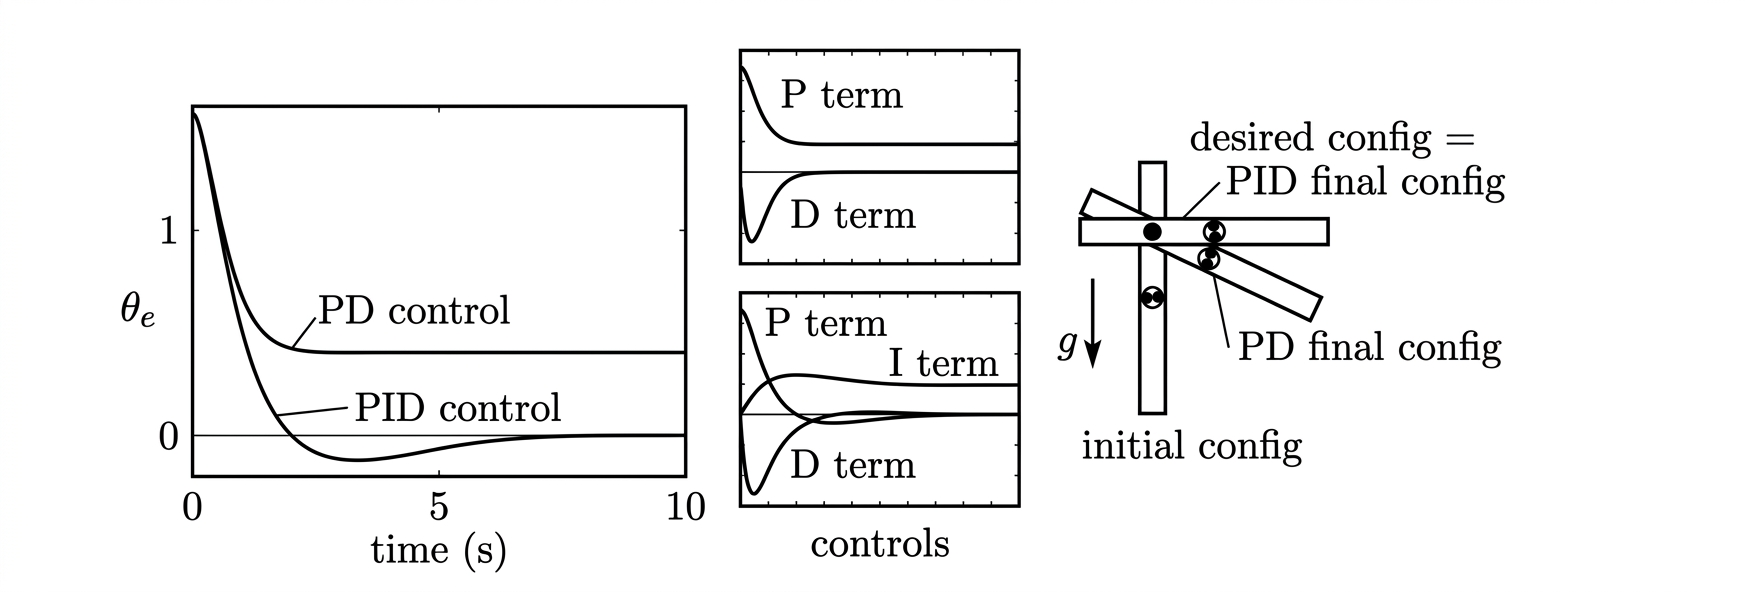
\includegraphics[width=0.8\linewidth]{img/pid.png}
\end{figure}

For attitude control, The error between the target orientation $q_{\text{target}}$ and the current body orientation $q_{\text{body}}$ is defined as \cref{eq:attitude}.

\begin{equation}\label{eq:attitude}
    \Delta q = q_{\text{target}} \cdot q_{\text{body}}^{-1}
\end{equation}

Using Unity's ToAngleAxis method, this relative rotation is converted into an angle $\phi$ and an axis $\mathbf{n}$. The error vector $\mathbf{e}$ is then $\mathbf{e} = \phi \cdot \mathbf{n}$.

The controller applies a PD loop (Proportional-Derivative) to generate corrective torque shown in \cref{eq:pdt}.

\begin{equation}\label{eq:pdt}
    \boldsymbol{\tau}_{\text{world}} = K_p \cdot \mathbf{e} + K_d \cdot \frac{\mathbf{e} - \mathbf{e}_{k-1}}{\Delta t}
\end{equation}

The world-space torque is transformed into the body frame ($R_{\text{wb}}$) for the physics simulation: $\boldsymbol{\tau}_{\text{body}} = R_{\text{wb}} \cdot \boldsymbol{\tau}_{\text{world}}$

The controller should be able to pilot the quadcopter in a closed-loop mission. The system employs a cascaded control scheme where the Outer Loop (Position) provides setpoints for the Inner Loop (Attitude/Velocity).

The Inner Loop features controllers that yield the required rolling and pitching moments $\tau_x$ and $\tau_y$ to regulate horizontal movement. The Inner Loop block requires the current quadcopter attitude as well as reference signals for roll and pitch to obtain its output \parencite{paredes2021quadcopter}; The Outer Loop, which features controllers that yield the required thrust differential and yawing moments as well as the desired reference signals.

During takeoff, the controller focuses exclusively on vertical error ($e_y$). The vertical force $force_Y$ is mapped to a normalized throttle value ($T$) shown in \cref{eq:mappingt}.

Following a path requires a look-ahead method. Given current position $\mathbf{p}$ and look-ahead target $\mathbf{t}$ on the path, the position error is defined as: $e_x = t_x - p_x,\quad e_y = t_y - p_y,\quad e_z = t_z - p_z$. 

The Outer Loop converts this error into a desired velocity in the world axis as shown in \cref{eq:outerLoop}.

\begin{equation}\label{eq:outerLoop}
    v_{x,\text{des}} = \text{PD}_X(e_x),\quad v_{z,\text{des}} = \text{PD}_Z(e_z)
\end{equation}

To translate these into drone-relative commands (Pitch/Roll), the world velocity is projected onto the drone's Heading Axis: (1) Forward Basis: $\hat{\mathbf{f}} = R_y(\psi)\,\hat{\mathbf{z}}_{\text{forward}}$; (2) Right Basis: $\hat{\mathbf{r}} = R_y(\psi)\,\hat{\mathbf{x}}_{\text{right}}$; The projections shown as \cref{eq:projection}. Where $e_{v,\parallel}$ is the longitudinal velocity error,  $e_{v,\perp}$ is the lateral velocity error.

\begin{equation}\label{eq:projection}
    v^{\parallel}_{\text{des}} = \mathbf{v}_{H,\text{des}}\cdot\hat{\mathbf{f}}, \quad v^{\perp}_{\text{des}} = \mathbf{v}_{H,\text{des}}\cdot\hat{\mathbf{r}}
\end{equation}

The Inner Loop then calculates the error between desired and actual velocity to produce stick inputs. Pitch (Right Vertical): Based on $e_{v,\parallel}$; Roll (Right Horizontal): Based on $e_{v,\perp}$.

The target yaw speed $\psi_{\text{target}} = \operatorname{atan2}(v_x,\,v_z)$, the yaw error is  $e_\psi = \text{DeltaAngle}(\psi, \psi_{\text{target}})$, so mapped to joystick movement is $u_{\text{yaw}} = \text{PID}_{\text{yaw}}(e_\psi)$. The other axis are the same methods.
\subsubsection{Design of a RL-Based HAC}

Alternatively, reinforcement learning (RL) can also be used in building an HAC agent with Unity's Machine Learning Agents (ML-Agents). ML-Agents allows developers to utilize games and simulations as training environments for intelligent agents. These agents can be trained using various paradigms, including reinforcement learning, imitation learning, and neuroevolution. Practical applications of trained agents encompass the control of non-player character (NPC) behavior in multi-agent or adversarial settings, automated game build testing, and the pre-release evaluation of game design decisions.

To facilitate training, a configuration file is typically required for the Python API, with Proximal Policy Optimization (PPO) serving as the predominant algorithm. The Python API interacts with the Unity environment via a communicator to execute the training process. Upon completion, the trained model is exported as an Open Neural Network Exchange (ONNX) file, which is subsequently used for agent inference and control. Furthermore, Unity provides a heuristic API for debugging and imitation learning (IL), enabling manual control over agents and the adjustment of training outcomes, as illustrated in \cref{fig:agent}.

\begin{figure}
    \caption{Simplified ML-Agents Scene Block Diagram}\label{fig:agent}
    \centering
\begin{tikzpicture}[
    font=\sffamily\bfseries,
    base/.style={rectangle, rounded corners=5pt, minimum width=2.2cm, minimum height=1cm, align=center, draw=white, line width=1pt, text=white},
    agent/.style={base, fill={rgb,255:red,119; green,184; blue,103}},
    behavior/.style={base, fill={rgb,255:red,98; green,155; blue,210}, minimum width=3cm},
    purple_box/.style={base, fill={rgb,255:red,146; green,106; blue,196}},
    orange_box/.style={base, fill={rgb,255:red,243; green,156; blue,87}},
    red_box/.style={base, fill={rgb,255:red,219; green,97; blue,94}},
    yellow_box/.style={base, fill={rgb,255:red,241; green,190; blue,47}},
    arrow/.style={<->, >=Stealth, thick, white},
    % 使用 * 并在连线时稍微偏移
    dash_arrow/.style={*-, dashed, thick, black} 
]

    % --- 内部节点 ---
    \node[behavior] (behA) {Behavior A};
    \node[agent, above left=1.5cm and -1.2cm of behA] (a1) {Agent\\A1};
    \node[agent, above right=1.5cm and -1.2cm of behA] (a2) {Agent\\A2};
    \node[orange_box, below=1cm of behA] (comm) {Communicator};

    \node[behavior, right=1cm of behA, minimum width=2.2cm] (behC) {Behavior C};
    \node[agent, at={(behC |- a1)}] (c1) {Agent\\C1};
    \node[purple_box, below=1cm of behC] (inf) {Inference};

    \node[behavior, right=1cm of behC, minimum width=2.2cm] (behD) {Behavior D};
    \node[agent, at={(behD |- a1)}] (d1) {Agent\\D1};
    \node[purple_box, below=1cm of behD] (heu) {Heuristic};

    % --- 外部节点 ---
    \node[red_box, below=2cm of comm] (pyAPI) {Python API};
    \node[yellow_box, right=1.2cm of pyAPI] (pyTrain) {Python Trainer};

    % --- 连线 ---
    \draw[arrow] (behA.north) -- ++(0,0.6) -| (a1.south);
    \draw[arrow] (behA.north) -- ++(0,0.6) -| (a2.south);
    \draw[arrow] (behA) -- (comm);
    \draw[arrow] (c1) -- (behC);
    \draw[arrow] (behC) -- (inf);
    \draw[arrow] (d1) -- (behD);
    \draw[arrow] (behD) -- (heu);
    
    % 虚线连线：起点从 comm.south 稍微往下移 1pt，确保圆点（*）不被框线切掉
    \draw[dash_arrow] ([yshift=-1pt]comm.south) -- (pyAPI.north);
    \draw[arrow, black] (pyAPI) -- (pyTrain);

    % --- 背景框 ---
    \begin{scope}[on background layer]
        % 增加 inner ysep=30pt 确保上下都有足够的留白
        \node[fill=gray, rounded corners=10pt, 
              fit=(a1) (a2) (c1) (d1) (comm) (inf) (heu), 
              inner xsep=15pt, inner ysep=30pt] (env) {};
        
        \node[anchor=north west, text=white, inner sep=10pt] at (env.north west) {Learning Environment};
    \end{scope}

\end{tikzpicture}
\end{figure}


For this research, each Drone Agent includes, (1) Agent Script, Handles OnActionReceived (processing joystick inputs), CollectObservations (monitoring states), and Heuristic (manual control for debugging); (2) Behavior Parameters: Defines the vector space for actions and observations. (3) Decision Requester: Controls the frequency of actions. By limiting the request rate, we can simulate more human-like reaction times, making the agent a better tutor for human pilots.

Proximal Policy Optimization (PPO) is an on-policy actor-critic algorithm that updates policies in small, clipped steps to ensure stability \parencite{openai2017ppo}. PPO is particularly effective for drones learning to navigate complex environments \parencite{yu2025depth}.

The optimization objective is defined as \cref{eq:ppo} shows.

\begin{equation}\label{eq:ppo}
L^{CLIP}(\theta) = \hat{\mathbb{E}}_t [ \min(r_t(\theta)\hat{A}_t, \text{clip}(r_t(\theta), 1-\epsilon, 1+\epsilon)\hat{A}_t) ]
\end{equation}

\begin{itemize}
    \item $\theta$ is the policy parameter
    \item $\hat{E}_t$ denotes the empirical expectation over timesteps
    \item $r_t$ is the ratio of the probability under the new and old policies, respectively
    \item $\hat{A}_t$ is the estimated advantage at time $t$
    \item $\epsilon$ is a hyperparameter, usually $0.1$ or $0.2$
\end{itemize}

Compared with a PID AI agent, a reinforcement learning-based AI agent does not require repeated testing to fine-tune parameters. Decisions are executed through a Decision Requester, which makes it easier to adjust the request frequency and pacing. However, as a black-box approach, it can be more difficult to achieve optimal performance or interpret and refine its behavior.

\subsubsection{Evaluation For the HAC Agents}

The evaluation strategy is designed to assess the performance of the Human-AI Collaboration (HAC) system in terms of control stability and trajectory tracking capability. Two representative control tasks were defined: a vertical hovering task and a synthetic path following task. These tasks were selected as simplified proxies to evaluate the underlying control effectiveness without requiring full mission complexity.

\paragraph{Hovering Task}

The hovering task evaluates the system's ability to maintain stable altitude control. The objective is to regulate the drone's vertical position ($y$) within a predefined tolerance band $[H - R, H + R]$, where $H$ represents the target altitude and $R$ defines the acceptable deviation range.

Performance is monitored through both positional stability and qualitative visual feedback. A color-coded indicator system is used to provide real-time feedback on control states: yellow indicates the drone is below the target range, orange indicates it is above the range, and blue indicates stable hovering within the acceptable band (see \cref{fig:train}). This visualization supports rapid assessment of control stability during operation.

\begin{figure}[H]
    \caption{Real-time feedback visualization during hovering evaluation.}\label{fig:train}
    \centering
    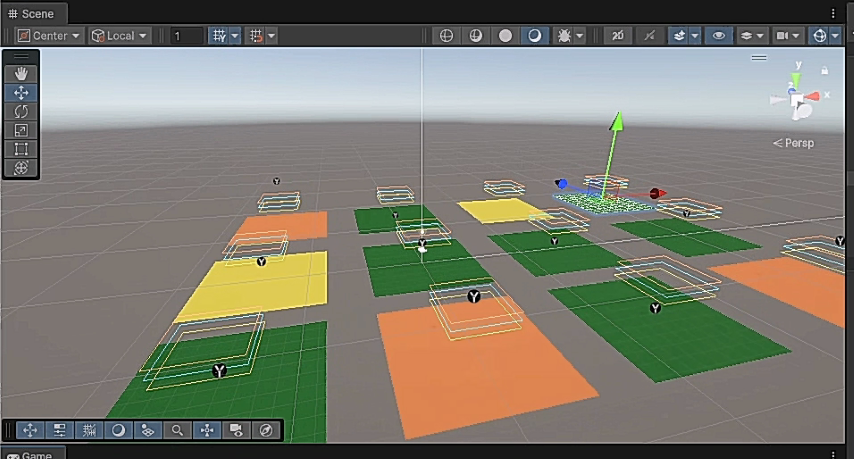
\includegraphics[width=0.8\linewidth]{img/train.png}
\end{figure}

The primary evaluation criterion for this task is the duration and consistency of maintaining the drone within the acceptable altitude band, which reflects the stability of the control system.

\paragraph{Path Following Task}

The path following task is introduced as a controlled synthetic trajectory tracking problem to evaluate the system's ability to follow predefined spatial references. This task is not intended to represent a realistic mission scenario, but rather to test the responsiveness and coordination of the control system under structured motion constraints.

A smooth trajectory is generated using cubic Bézier curves defined by four control points $P_0, P_1, P_2, P_3$, forming a round-trip path from the home position to a target waypoint and back. The trajectory is defined as:

\begin{equation}\label{eq:bezier}
    B(t) = {(1-t)}^3 P_0 + 3{(1-t)}^2 t P_1 + 3(1-t) t^2 P_2 + t^3 P_3, \quad t \in [0,1]
\end{equation}

The resulting path provides a continuous reference trajectory for evaluating tracking behavior. The geometric structure of the generated path is shown in \cref{fig:path_design}, where asymmetric control point offsets are used to create directional variation between outbound and return segments.

\begin{figure}[H]
    \caption{Synthetic path structure used for trajectory tracking evaluation.}\label{fig:path_design}
    \centering
    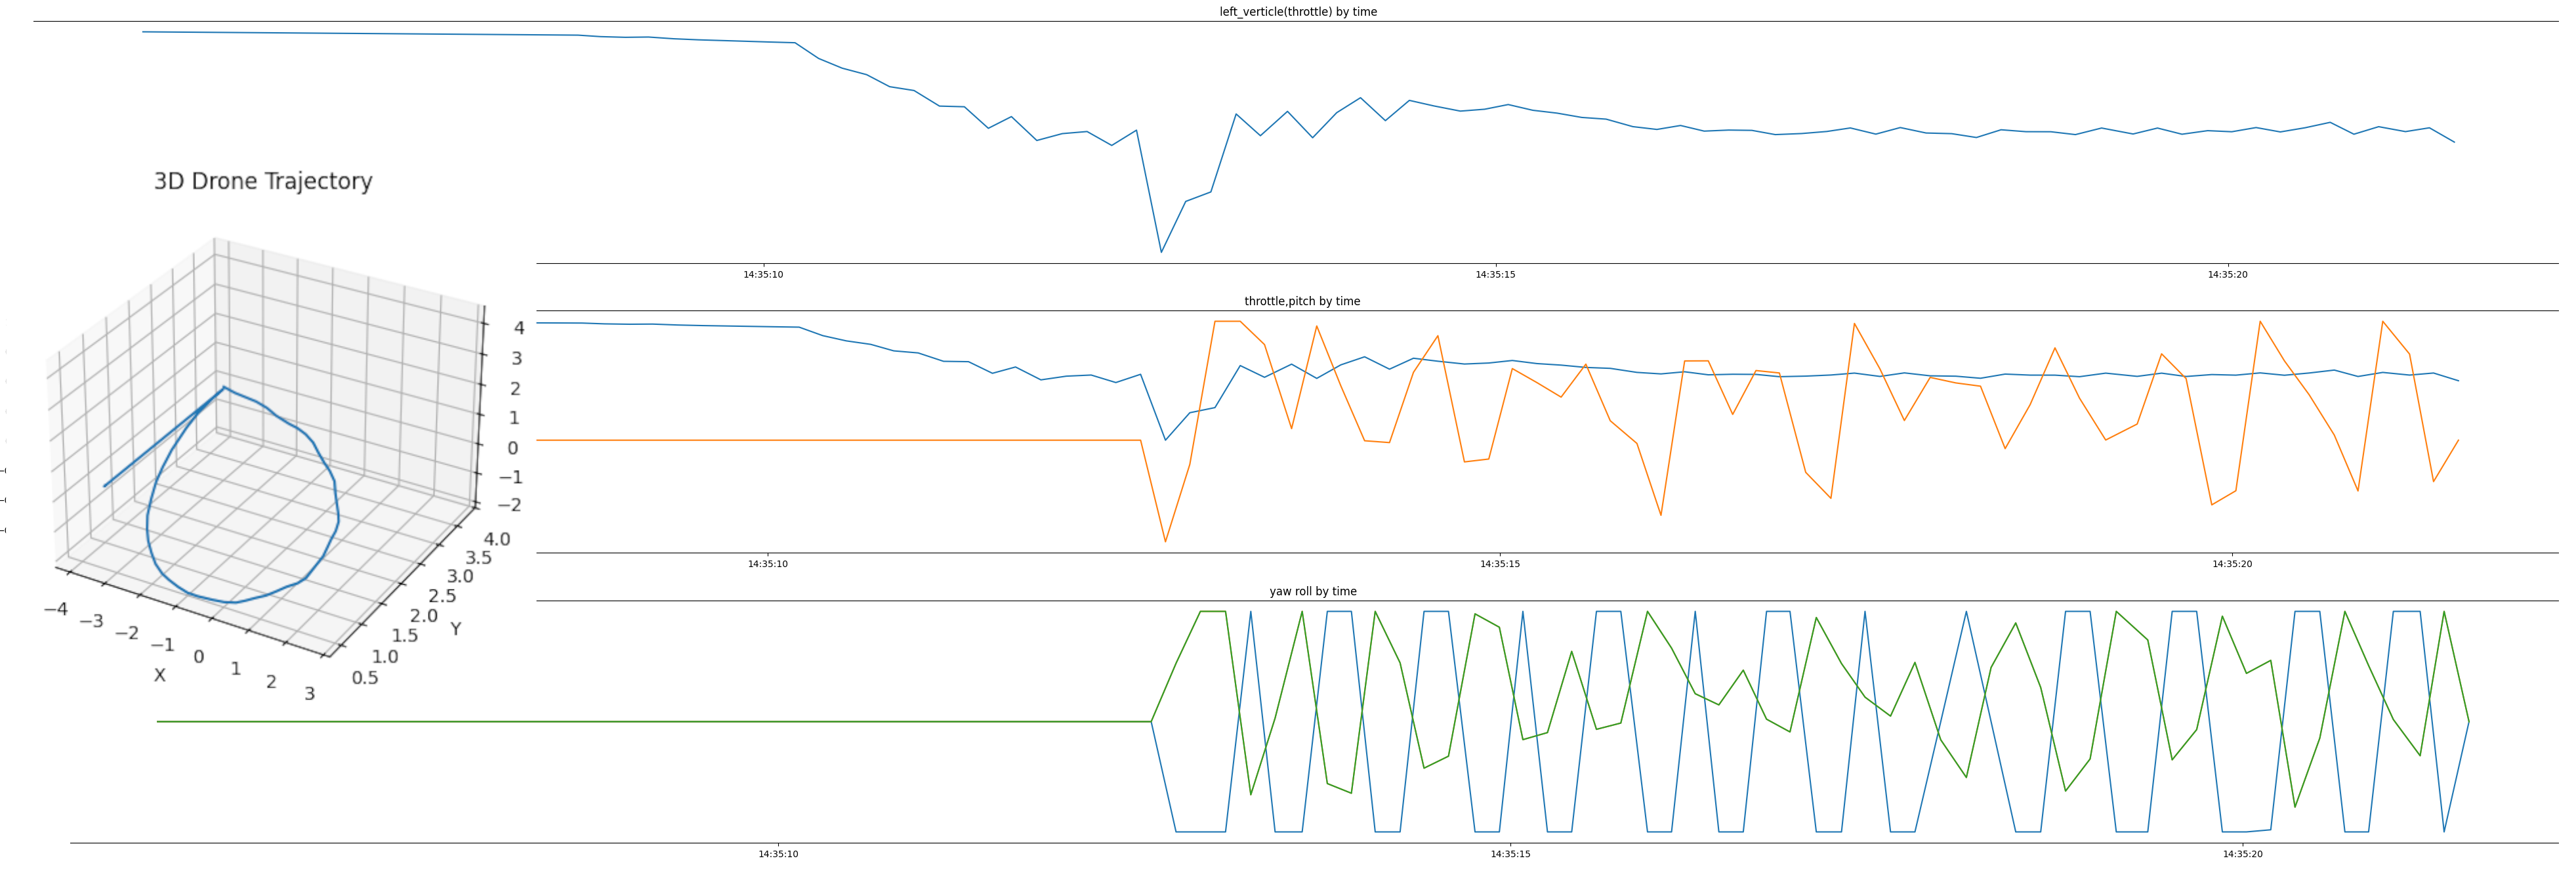
\includegraphics[width=0.8\linewidth]{img/path.png}
\end{figure}

Evaluation in this task focuses on trajectory tracking performance, including deviation from the reference path and stability of directional control during transitions between waypoints. 

\paragraph{Evaluation Environment}

To ensure consistent comparison across tasks, both hovering and path following evaluations are conducted in a non-XR visualization environment. System behavior is projected onto a flat-panel interface, allowing direct observation of control signals and system responses without requiring immersive hardware. This setup ensures reproducibility and simplifies performance analysis across experimental runs.

% Object: XR interactions

\subsection{Comparison of Current XR Development Platforms}

XR development is heavily dictated by the choice of game engine. Before initiating a project, it is critical to determine the target hardware and environmental requirements, as these factors define the development constraints.


% <!-- TODO: move to theory or other places
Mixed reality (MR) headsets create immersive experiences designed to spatially integrate virtual content into the physical world. The newest headsets rely on passthrough video. While using passthrough, a person does not see light from the real world but instead relies on stereoscopic, color, high resolution, low latency, real-time video of the world, which is displayed on small screens inside a headset \parencite{bailenson2024passthrough}.

\parencite{waldow_investigating_2025} investigates Pass-Through Embodiment (PTE), The study found that PTE significantly enhances the user's sense of presence and embodiment compared to using a customizable digital avatar. The ability to see one's own body strengthens the feeling of being physically present in the VR environment without negatively affecting performance or causing sickness.

Leveraging passthrough on modern XR devices can help developers build highly engaging mixed-reality environments, which is particularly beneficial for applications like prototyping drone simulations.

% -->
Here, we present a comparison of current game engines that support extended reality, based on programming language, physics engine, rendering methods, Meta support, machine learning support, and editor size (see Table~\ref{table:xr_engine}).

\begin{table}[h]
\centering
\caption{Software Engine Comparison}\label{table:xr_engine}
\setlength{\tabcolsep}{6pt} 
\begin{tabularx}{1\textwidth}{l|X|X|X|X}
\hline
Feature & Unreal Engine (5.7) & Unity (6.0) & Godot (4.6) & Wonderland Engine \\
\hline
Language & C++, Blueprints    & C\#        & GDScript, C\# & JavaScript, TypeScript \\
Physics & Chaos Physics      & NVIDIA PhysX, DOTS & Jolt Physics   & NVIDIA PhysX \\
Rendering  & Lumen, Nanite & URP, HDRP    & Forward+, Mobile & WebGL2 \\
Meta Support & Fork build  & First-class & Community-driven & No support \\
ML Support & Learning Agent & ML Agents & Godot RL Agents & No support \\
Editor Size & $\sim$50GB+ & $\sim$20GB & $<1$GB & 200MB \\
\hline
\end{tabularx}

\end{table}

Unreal Engine: UE is known for photorealistic rendering, UE provides unparalleled visual fidelity. Its Chaos Physics engine is highly regarded for complex simulations, making it the foundation for projects like Microsoft's AirSim. However, UE has a high barrier to entry: the editor is massive, and utilizing Meta's private APIs often requires compiling a custom engine branch from source.

Unity: Unity remains the most popular choice for Meta Quest development due to its mature SDK support and C\# scripting. While it uses PhysX by default, its DOTS (Data-Oriented Technology Stack) provides high-performance physics for complex drone swarms. It offers the most streamlined out-of-the-box experience for Standalone VR.

Godot: Godot has emerged as a powerful, lightweight alternative. It is highly compatible with modern AI coding assistants due to its Python-like GDScript. The integration of Jolt Physics as the default 3D engine has resolved previous performance hurdles for VR. However, its XR ecosystem is largely community-maintained. While excellent for prototyping, the lack of official Meta API support and the potential instability of third-party GDExtensions require careful dependency management for production-grade projects.

Wonderland Engine: Wonderland Engine is a specialized WebXR engine built in C++ and compiled to WebAssembly.  By leveraging WebGL2, it achieves the performance necessary to render thousands of objects at native frame rates directly within a browser. The development workflow relies on JavaScript and TypeScript, providing a highly familiar and accessible environment for traditional web developers. A unique advantage is the ability to edit scenes directly on the headset, enabling instant feedback without removing the device.




\subsection{Participants and Testing Environment}

The formative evaluation involved the researcher and a small number of voluntary participants (N = 3). Participants were primarily virtual reality enthusiasts who owned a Meta Quest headset and did not necessarily have prior experience with FPV drone control. Participant involvement was not strictly controlled across iterations; instead, feedback was collected opportunistically from available users at different stages of development. The purpose of participant involvement was to gather diverse usability perspectives rather than to support comparative or statistical analysis.

The system was developed on a laptop computer equipped with an Intel 13th Gen i9 processor, 64 GB RAM, and an NVIDIA RTX 4070 GPU. The application was deployed and tested on Meta Quest 3 and Meta Quest 3S devices using standalone execution, without reliance on PCVR streaming.

